\documentclass[12pt,a4paper]{article}
\usepackage[top=2.5cm,bottom=2.5cm,left=2.5cm,right=2.5cm]{geometry}
\usepackage{graphicx}
\usepackage{amsmath}
\usepackage{amssymb}
\usepackage{booktabs}
\usepackage{caption}
\usepackage{subcaption}
\usepackage{float}
\usepackage{hyperref}
\usepackage{enumitem}
\usepackage{setspace}
\usepackage{titlesec}

\titlespacing*{\section}{0pt}{10pt}{4pt}
\titlespacing*{\subsection}{0pt}{8pt}{3pt}
\setlength{\parskip}{4pt}
\setlength{\parindent}{1em}
\setstretch{1.15}

% ── Fill in your details ───────────────────────────────────────────────────
\newcommand{\MyName}{[Your Name]}
\newcommand{\MySupervisor}{[Supervisor Name]}
\newcommand{\MyCourse}{[Course Name]}
\newcommand{\MyDate}{[Date / Time]}
\newcommand{\MyLocation}{[Location]}
% ──────────────────────────────────────────────────────────────────────────

\begin{document}

% ── Header ─────────────────────────────────────────────────────────────────
\begin{center}
  {\LARGE\bfseries Lightweight Visual Navigation Policy for UAVs via\\[4pt]
  Knowledge Distillation from a Classical Autonomy Stack}\\[10pt]
  {\large \MyName}\\[4pt]
  Supervisor: \MySupervisor \quad Course: \MyCourse\\[2pt]
  \MyDate \quad \MyLocation
\end{center}

\vspace{6pt}
\noindent\textbf{Abstract.}~%
This report presents an ongoing study on transferring autonomy knowledge from a
classical UAV planning and control stack to a lightweight, front-camera-only
visual navigation policy through knowledge distillation (KD).
The teacher is the CERLAB Autonomous Flight system, which uses
depth perception, B-spline trajectory planning, and a tracking controller.
The student is a compact MobileNetV2-based network that must navigate using only
a monocular front camera at deployment.
Four distillation strategies are designed: a behavior cloning baseline~(BC),
trajectory-level KD~(TrajKD), self-predicted waypoint with curriculum learning~(SelfRedWP),
and the proposed Joint KD~(JointKD) that combines planning-level and
execution-level supervision.
Offline evaluation on the \texttt{uav\_kd\_v002} dataset shows that
planning-level supervision consistently reduces yaw-rate prediction error
relative to the no-KD baseline, with SelfRedWP achieving the lowest
per-dimension control MSE among currently trained methods.
Training of CtrlKD and JointKD is in progress.

\vspace{4pt}
\noindent\textbf{Keywords:}~knowledge distillation, UAV, behavior cloning,
visual navigation policy, trajectory prediction, curriculum learning, MobileNetV2.

% ── 1. Introduction ─────────────────────────────────────────────────────────
\section{Introduction}

Classical UAV autonomy stacks achieve reliable navigation by fusing rich sensor
modalities---LiDAR, depth cameras, HD maps, and inertial odometry---into
sophisticated planning pipelines.
These stacks, however, are too heavy for payload-limited platforms and cannot
operate in sensor-degraded or map-free environments.
End-to-end visual policies trained via imitation learning offer compactness and
generality, but naive behavior cloning~(BC) from expert demonstrations often
fails to capture the hierarchical structure of the expert's decision making~\cite{Ross2011}.

Knowledge distillation~\cite{Hinton2015} provides a principled framework for
transferring the internal ``knowledge'' of a complex teacher into a compact student.
Rather than imitating only the final control output, the student can be trained to
reproduce intermediate representations such as planned trajectories and multi-step
control sequences, thereby gaining the teacher's planning intent alongside its
reactive control skill.

This work investigates \emph{what level of teacher knowledge} is most beneficial
to distill into a lightweight UAV visual policy, by designing and comparing
four distillation strategies under a unified evaluation protocol.

% ── 2. Teacher System ───────────────────────────────────────────────────────
\section{Teacher System}

The teacher is the CERLAB Autonomous Flight system running in the Gazebo simulator.
It consists of three modules: (i) a depth-based perception module that extracts
occupancy information from depth images and LiDAR point clouds;
(ii) a B-spline trajectory planner that generates smooth, collision-free future paths;
and (iii) a tracking controller that converts the planned trajectory into velocity
commands $\mathbf{u}_t = [v_x, v_y, v_z, \dot{\psi}]$.

Two types of teacher signals are recorded for distillation:
\begin{itemize}[noitemsep,topsep=2pt]
  \item \textbf{Control label} $\mathbf{u}_t$: the 4-DOF velocity command at each frame.
  \item \textbf{Trajectory label} $\boldsymbol{\tau}_t$: a sequence of $K{=}10$ future
        waypoints in the UAV body frame,
        $\boldsymbol{\tau}_t = \{(\Delta x_k, \Delta y_k, \Delta z_k)\}_{k=1}^{K}$.
\end{itemize}
Both signals are synchronized with the front-camera image stream at 20\,Hz and
stored as processed dataset samples.

% ── 3. Student Model Architecture ──────────────────────────────────────────
\section{Student Model Architecture}

\begin{figure}[H]
  \centering
  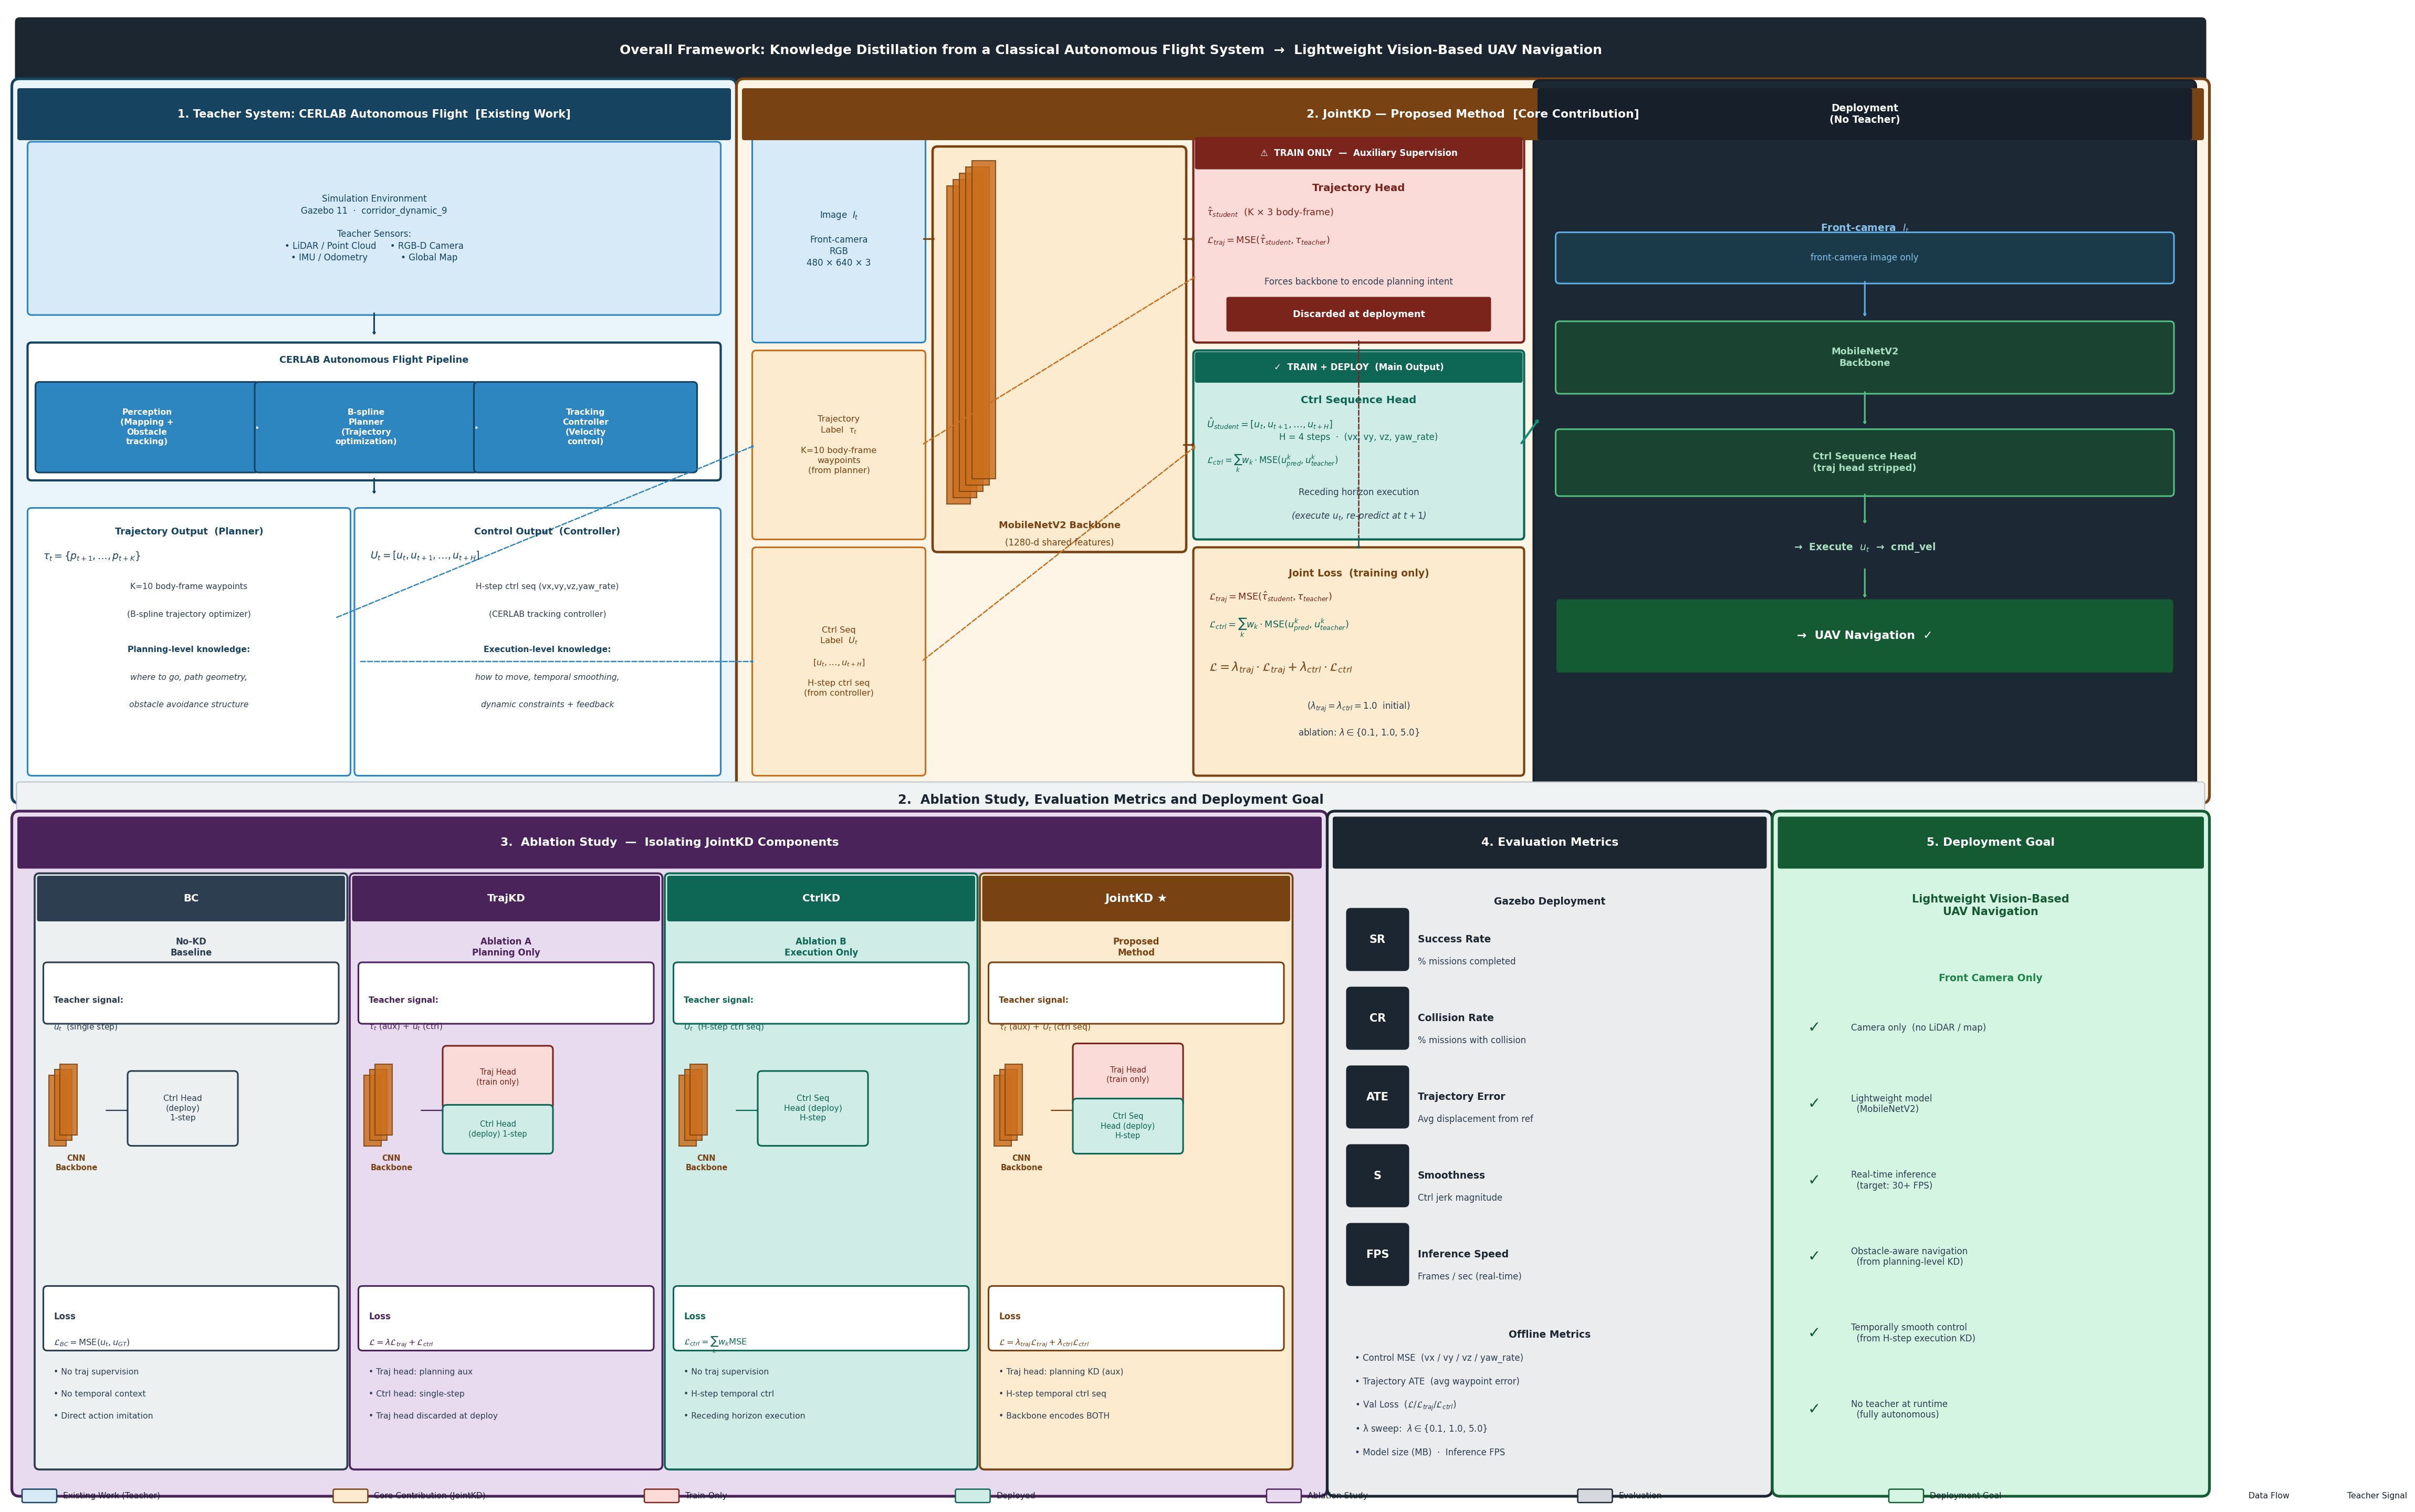
\includegraphics[width=\linewidth]{framework_overview.png}
  \caption{Overall framework. \emph{Top row:} teacher system (blue) and proposed JointKD student (orange/teal).
           The trajectory head (red, train-only) is discarded at deployment; only the control sequence head (teal) runs on-device.
           \emph{Bottom row:} ablation variants (purple) and evaluation pipeline (navy/green).}
  \label{fig:framework}
\end{figure}

The student backbone is \textbf{MobileNetV2}~\cite{Sandler2018} pretrained on
ImageNet, producing a 1280-dimensional feature vector from a $224{\times}224$
RGB front-camera image.
All distillation variants share this backbone; they differ only in the prediction
heads attached to it.
At deployment, the student receives only the front-camera image---no LiDAR,
depth camera, map, or odometry is available.

Two types of prediction heads are used:
\begin{itemize}[noitemsep,topsep=2pt]
  \item \textbf{Control head}: a 2-layer MLP (1280\,$\to$\,256\,$\to$\,$4{\times}H$)
        that predicts either a single-step command ($H{=}1$) or an $H$-step control
        sequence.
  \item \textbf{Trajectory head}: a 2-layer MLP (1280\,$\to$\,256\,$\to$\,$K{\times}3$)
        that predicts the $K{=}10$ future waypoints; used only as an auxiliary
        training head and discarded at deployment.
\end{itemize}

% ── 4. Knowledge Distillation Methods ──────────────────────────────────────
\section{Knowledge Distillation Methods}

\subsection{Behavior Cloning Baseline (BC)}
The baseline directly maps the front-camera image to a single-step control command
without any trajectory supervision:
\begin{equation}
  \mathcal{L}_{\text{BC}} = \|\hat{\mathbf{u}}_t - \mathbf{u}_t\|^2_2
\end{equation}
This corresponds to standard behavior cloning~\cite{Pomerleau1989} and serves as
the no-KD reference point.

\subsection{Trajectory-Level KD (TrajKD)}
TrajKD attaches both a trajectory head and a control head to the shared backbone.
The trajectory head is supervised by the teacher's planned waypoints, providing an
auxiliary planning-level loss:
\begin{equation}
  \mathcal{L}_{\text{TrajKD}} = \lambda_{\text{traj}}\,\mathcal{L}_{\text{traj}}
  + \mathcal{L}_{\text{ctrl}},
  \quad
  \mathcal{L}_{\text{traj}} = \frac{1}{K}\sum_{k=1}^{K}\|\hat{\boldsymbol{\tau}}_k - \boldsymbol{\tau}_k\|^2_2
\end{equation}
At deployment, the trajectory head is discarded and only the control head produces
output.
This design forces the backbone to encode planning intent into its features,
which is then exploited by the control head.

\subsection{Self-Predicted Waypoint with Curriculum (SelfRedWP)}
TrajKD introduces a \emph{train-deploy mismatch}: at training time the trajectory
head is supervised by ground-truth teacher waypoints, but at deployment it would
receive its own (potentially imperfect) predictions.
SelfRedWP resolves this by rendering the predicted waypoint as a red dot overlay
on the input image, making the planning signal \emph{explicit} rather than implicit.

A curriculum schedule gradually transitions the red-dot source from the ground-truth
teacher waypoint (epoch 1--5) to the model's own predicted waypoint (epoch 5--35,
linear ramp), reaching full self-prediction at epoch 35 and maintaining it thereafter.
This mirrors DAgger-style on-policy training~\cite{Ross2011} without requiring
environment interaction.

\subsection{Control Sequence KD (CtrlKD)}
CtrlKD distills the teacher's \emph{execution} knowledge by supervising an
$H$-step future control sequence:
\begin{equation}
  \mathcal{L}_{\text{CtrlKD}}
  = \sum_{h=0}^{H-1} w_h\,\|\hat{\mathbf{u}}_{t+h} - \mathbf{u}_{t+h}\|^2_2
\end{equation}
At deployment, the model predicts $H$ steps and executes only $\mathbf{u}_t$,
re-predicting at every frame (receding-horizon execution).
This ablation isolates whether execution-level temporal consistency
improves over single-step BC without any planning supervision.
Training is in progress ($H{=}5$, uniform weights $w_h{=}1$).

\subsection{Joint KD (JointKD) — Proposed Method}
JointKD combines both levels of teacher knowledge:
\begin{equation}
  \mathcal{L}_{\text{JointKD}}
  = \lambda_{\text{traj}}\,\mathcal{L}_{\text{traj}}
  + \lambda_{\text{ctrl}}\,\mathcal{L}_{\text{ctrl\_seq}}
\end{equation}
The trajectory head provides planning regularisation; the $H$-step control
sequence head is deployed with receding-horizon execution.
The trajectory head is stripped from the checkpoint before deployment.
Initial hyperparameters: $\lambda_{\text{traj}}{=}1.0$,
$\lambda_{\text{ctrl}}{=}1.0$, $H{=}5$, $K{=}10$.
Training is in progress.

% ── 5. Dataset ──────────────────────────────────────────────────────────────
\section{Dataset}

The \texttt{uav\_kd\_v002} dataset comprises 7 flight episodes
(ep\_003--ep\_009) recorded in a Gazebo corridor environment.
Episodes ep\_001 and ep\_002 were excluded due to a coordinate-frame bug in
trajectory labelling.
The train/validation split is performed at the \emph{episode level} to avoid
data leakage from temporally adjacent frames.
Table~\ref{tab:dataset} summarises the dataset statistics.

\begin{table}[H]
\centering
\caption{Dataset summary for \texttt{uav\_kd\_v002}.
Rotation frames are defined as $|\dot{\psi}|>0.15$\,rad/s.}
\label{tab:dataset}
\small
\begin{tabular}{lrrrl}
\toprule
Episode & Frames & Rotation (\%) & Split & Note \\
\midrule
ep\_003 & 1013 & 0.0  & train & straight-flight only \\
ep\_004 &  958 & 0.0  & train & straight-flight only \\
ep\_007 & 4406 & 22.9 & train & longest; main turning source \\
ep\_008 & 2457 & 4.2  & train & mixed \\
ep\_009 & 1337 & 6.2  & train & mixed \\
ep\_005 &  569 & 0.0  & val   & straight-flight reference \\
ep\_006 &  962 & 18.2 & val   & rotation-inclusive val set \\
\bottomrule
\multicolumn{5}{l}{\small Total training: 6004--6722 frames (varies by split); val: 861--935 frames.}
\end{tabular}
\end{table}

% ── 6. Experimental Results ─────────────────────────────────────────────────
\section{Experimental Results}

All models are trained for 50 epochs using AdamW with a cosine-annealing
learning rate schedule (initial LR $= 1{\times}10^{-4}$, minimum $\approx 1{\times}10^{-7}$).

\begin{figure}[H]
  \centering
  \begin{subfigure}[b]{0.49\linewidth}
    
\includegraphics[width=\linewidth]{../results/figures/metric_plots/ctrl_dim_mse_v002.png}
    \caption{Per-dimension control MSE at best-val epoch.}
    \label{fig:dim_mse}
  \end{subfigure}
  \hfill
  \begin{subfigure}[b]{0.49\linewidth}
    
\includegraphics[width=\linewidth]{../results/figures/metric_plots/yr_learning_curves.png}
    \caption{Yaw-rate validation MSE over training.}
    \label{fig:yr}
  \end{subfigure}
  \caption{Offline evaluation results for v002 methods.}
  \label{fig:results}
\end{figure}

Table~\ref{tab:results} reports the validation metrics at each method's best
epoch.
The per-dimension MSE comparison in Fig.~\ref{fig:dim_mse} highlights three
observations.
First, $v_z$ (vertical velocity) is near zero for all methods, as the dataset is
predominantly level flight and provides no useful learning signal for this dimension.
Second, \textbf{yaw\_rate} is the hardest dimension; its MSE is an order of
magnitude larger than $v_y$, reflecting the difficulty of predicting turning
intent from a single image.
Third, both TrajKD and SelfRedWP reduce yaw-rate MSE relative to BC-v002
(Fig.~\ref{fig:yr}), confirming that trajectory-level planning supervision injects
directional intent into the backbone features.
SelfRedWP achieves the largest improvement (yr MSE~$= 0.0737$, a $16\%$ reduction
over BC-v002's $0.0879$), demonstrating the benefit of the curriculum that
closes the train-deploy gap on the red-dot waypoint.

\begin{table}[H]
\centering
\caption{Validation metrics at best-val epoch. ATE: average trajectory error.
         ``--'' denotes methods without a trajectory head.
         CtrlKD and JointKD are pending.}
\label{tab:results}
\small
\begin{tabular}{lcccccccc}
\toprule
Method & Best & \multicolumn{4}{c}{Control MSE} & ATE & Train \\
       & Val  & $v_x$ & $v_y$ & $v_z$ & yaw\_rate & (m) & setup \\
\midrule
BC-v002   & 0.0526 & 0.1014 & 0.0209 & 0.0000 & 0.0879 & -- & ctrl only \\
TrajKD    & 0.0885 & 0.0866 & 0.0227 & 0.0001 & 0.0835 & 0.2604 & ctrl+traj \\
SelfRedWP & 0.0843 & 0.0823 & 0.0215 & 0.0000 & \textbf{0.0737} & 0.2621 & ctrl+traj+curric. \\
CtrlKD    & -- & \multicolumn{6}{c}{(training in progress)} \\
JointKD   & -- & \multicolumn{6}{c}{(training in progress)} \\
\bottomrule
\multicolumn{8}{l}{\small Note: BC-v002 val loss = ctrl MSE only; TrajKD/SelfRedWP val loss = ctrl+$\lambda$\,traj (not directly comparable).}
\end{tabular}
\end{table}

% ── 7. Discussion ───────────────────────────────────────────────────────────
\section{Discussion}

\textbf{Effect of planning supervision.}
TrajKD and SelfRedWP both improve yaw-rate prediction relative to BC, supporting
the hypothesis that planning-level KD encodes turning intent into the backbone.
However, the trajectory head also inflates the total validation loss, and TrajKD
shows more oscillation than BC, suggesting that the dual-head objective introduces
variance with the current dataset size ({\raise.17ex\hbox{$\scriptstyle\sim$}}6000 training frames).

\textbf{Benefit of the curriculum.}
SelfRedWP outperforms TrajKD on yaw-rate and achieves a smoother late-training
validation curve.
The curriculum progressively closes the train-deploy gap by shifting supervision
from the ground-truth teacher waypoint to the model's own predicted waypoint,
analogous to DAgger~\cite{Ross2011} without requiring live simulation rollouts.

\textbf{Overfitting.}
All three trained methods exhibit a large train--val gap (train loss $\approx0.002$;
val loss $\approx0.05$--$0.09$), indicating overfitting on the current 7-episode dataset.
This motivates collecting additional episodes, applying stronger image augmentation,
and revisiting regularisation hyperparameters.

\textbf{Expected contribution of CtrlKD and JointKD.}
CtrlKD's $H$-step sequence distillation should introduce temporal smoothness
constraints that further reduce yaw-rate oscillation.
JointKD, by combining both levels of supervision, is expected to yield the best
overall control accuracy while maintaining the compactness of the student model.

% ── 8. Conclusion ───────────────────────────────────────────────────────────
\section{Conclusion and Future Work}

This report described a knowledge distillation framework for training a lightweight
front-camera UAV policy from a classical autonomy stack.
The core contribution is the hierarchical distillation design: trajectory-level
supervision (TrajKD, SelfRedWP) transfers planning intent, execution-level
supervision (CtrlKD) transfers temporal smoothness, and Joint KD (proposed)
combines both.
Current offline results confirm that planning-level KD reduces yaw-rate prediction
error, and that the SelfRedWP curriculum improves generalisation.

Next steps are: (1) complete CtrlKD and JointKD training; (2) run Gazebo deployment
ablation comparing all four methods; (3) expand the dataset to mitigate overfitting;
(4) produce the final offline and deployment comparison tables for the thesis.

% ── References ──────────────────────────────────────────────────────────────
\begin{thebibliography}{9}

\bibitem{Hinton2015}
G.~Hinton, O.~Vinyals, and J.~Dean,
``Distilling the Knowledge in a Neural Network,''
\textit{arXiv preprint arXiv:1503.02531}, 2015.

\bibitem{Sandler2018}
M.~Sandler, A.~Howard, M.~Zhu, A.~Zhmoginov, and L.-C.~Chen,
``MobileNetV2: Inverted Residuals and Linear Bottlenecks,''
in \textit{Proc. IEEE/CVF Conf. on Computer Vision and Pattern Recognition (CVPR)},
pp.~4510--4520, 2018.

\bibitem{Pomerleau1989}
D.~A.~Pomerleau,
``ALVINN: An Autonomous Land Vehicle in a Neural Network,''
in \textit{Advances in Neural Information Processing Systems (NeurIPS)},
vol.~1, pp.~305--313, 1989.

\bibitem{Ross2011}
S.~Ross, G.~Gordon, and D.~Bagnell,
``A Reduction of Imitation Learning and Structured Prediction to No-Regret Online Learning,''
in \textit{Proc. 14th Int. Conf. on Artificial Intelligence and Statistics (AISTATS)},
pp.~627--635, 2011.

\bibitem{Mellinger2011}
D.~Mellinger and V.~Kumar,
``Minimum Snap Trajectory Generation and Control for Quadrotors,''
in \textit{Proc. IEEE Int. Conf. on Robotics and Automation (ICRA)},
pp.~2520--2525, 2011.

\bibitem{Bojarski2016}
M.~Bojarski, D.~Del Testa, D.~Dworakowski, B.~Firner, B.~Flepp, P.~Goyal,
L.~D.~Jackel, M.~Monfort, U.~Muller, J.~Zhang, X.~Zhang, J.~Zhao, and K.~Zieba,
``End to End Learning for Self-Driving Cars,''
\textit{arXiv preprint arXiv:1604.07316}, 2016.

\end{thebibliography}

\end{document}
